\chapter{Implementation on Current Hardware}

\section{Software Architecture}

This section will serve as an overview of the current system software architecture and will provide an in-depth analysis of how the current ROS2 Node structure works.

\subsection{ROS 2 System Architecture}

The current system's ROS 2 architecture is composed of four primary nodes, each responsible for specific functionalities:

\begin{itemize}
    \item \textbf{MTM Node (Micro-ROS):} This node is responsible for streaming sensor data from the Master Tool Manipulator (MTM) and performing forward kinematics calculations to determine the target pose.
    \item \textbf{System Model Node:} This node maintains a Simulation Description Format (SDF) model of the MTM. It facilitates real-time visualization of the system's configuration and enables the calculation of various joint frames.
    \item \textbf{Joint Publisher Node:} Acting as an intermediary, this node utilizes the SDF model to offer an alternative method for calculating the target position based on TF (Transform Frame) transformations.
    \item \textbf{PSM Node (Micro-ROS):} This node handles sensor data acquisition, implements control logic, and drives the Patient Side Manipulator (PSM) system.
\end{itemize}

\begin{figure}[h!]
    \centering
    \begin{tikzpicture}[node distance=1cm, auto] % Reduced node distance for a narrower figure
        % Nodes
        \node (mtm) [block] {MTM Node};
        \node (sdf) [block, right=of mtm] {SDF Model};
        \node (jointpub) [block, right=of sdf] {Joint Publisher Node};
        \node (psm) [block, right=of jointpub] {PSM Node};

        % Arrows
        \draw[arrow] (mtm) -- (sdf);
        \draw[arrow] (sdf) -- (jointpub);
        \draw[arrow] (jointpub) -- (psm);
    \end{tikzpicture}
    \caption{Initial ROS 2 System Architecture for Target Pose Calculation.}
    \label{fig:initial_architecture}
\end{figure}

Initially, the research aimed for the MTM Node to relay its joint angles to the SDF Model of the MTM. Subsequently, the Joint Publisher Node would calculate the desired end-effector position via a TF frame transformation from the base frame to the gimbal origin. This approach was intended to provide an alternative method for extracting the target position, bypassing the need for explicit forward kinematics in the MTM node. This architecture is illustrated in Figure \ref{fig:initial_architecture}. While this method proved effective in accurately calculating the target pose, real-time performance trials revealed significant limitations.

Specifically, although the target position extracted from the model demonstrated excellent real-time performance, a communication protocol breakdown was observed when the Joint Publisher Node interfaced with the Micro-ROS PSM Node. This breakdown was likely caused by memory limitations inherent to the Teensy 4.1 microcontroller, leading to high latency and noticeable data stuttering.

---

Consequently, a simplified architecture was explored to overcome these real-time performance issues. This revised approach involves performing forward kinematics calculations of the target position directly within the MTM Node and streaming this data topic directly to the PSM Node. This simplification of the technical stack significantly improved real-time performance and reduced system complexity. This optimized architecture is presented in Figure \ref{fig:optimized_architecture}.

\begin{figure}[h!]
    \centering
    \begin{tikzpicture}[node distance=2.5cm, auto]
        % Nodes
        \node (mtm) [block] {MTM Node};
        \node (psm) [block, right=of mtm] {PSM Node};

        % Arrows
        \draw[arrow] (mtm) -- (psm);
    \end{tikzpicture}
    \caption{Optimized ROS 2 System Architecture for Direct Target Pose Streaming.}
    \label{fig:optimized_architecture}
\end{figure}

\subsection{MTM Modeling and Visualization}

For the modeling of the MTM, the Simulation Description Format (SDF) was chosen due to its compatibility with ROS 2 and RViz. SDF also supports complex kinematic structures, including closed-chain kinematics, which is crucial for accurately modeling the more intricate four-bar style linkages found in the Patient Side Manipulator (PSM).

Generating the SDF file proved to be a fairly involved process. First, the CAD model of the MTM system was imported into SolidWorks. To reduce computational complexity, the model underwent significant simplification. Parts were condensed into their respective links, identified as follows:

\begin{itemize}
    \item Base
    \item J1 (Joint 1)
    \item J2 (Joint 2)
    \item J3 (Joint 3)
    \item G3 (Gimbal Link 3)
    \item G2 (Gimbal Link 2)
    \item G1 (Gimbal Link 1)
    \item G0 (Gimbal Link 0)
\end{itemize}

Each of these components was created as a singular solid part and then reassembled within SolidWorks into a complete assembly.

Following this, rotational axes and origins were assigned for each link. A SolidWorks plugin was then utilized to export the model into a Universal Robot Description Format (URDF) file. This URDF file was subsequently converted to SDF using a dedicated software tool, \textit{ros2\_sdf\_to\_urdf} (further citation needed). Upon the successful generation of the SDF model, a Python launch file was developed to facilitate quick and easy visualization of this model within RViz.

The final result of this effort can be seen below in Figure \ref{fig:mtm_sdf_model}.

\begin{figure}[h]
    \centering
    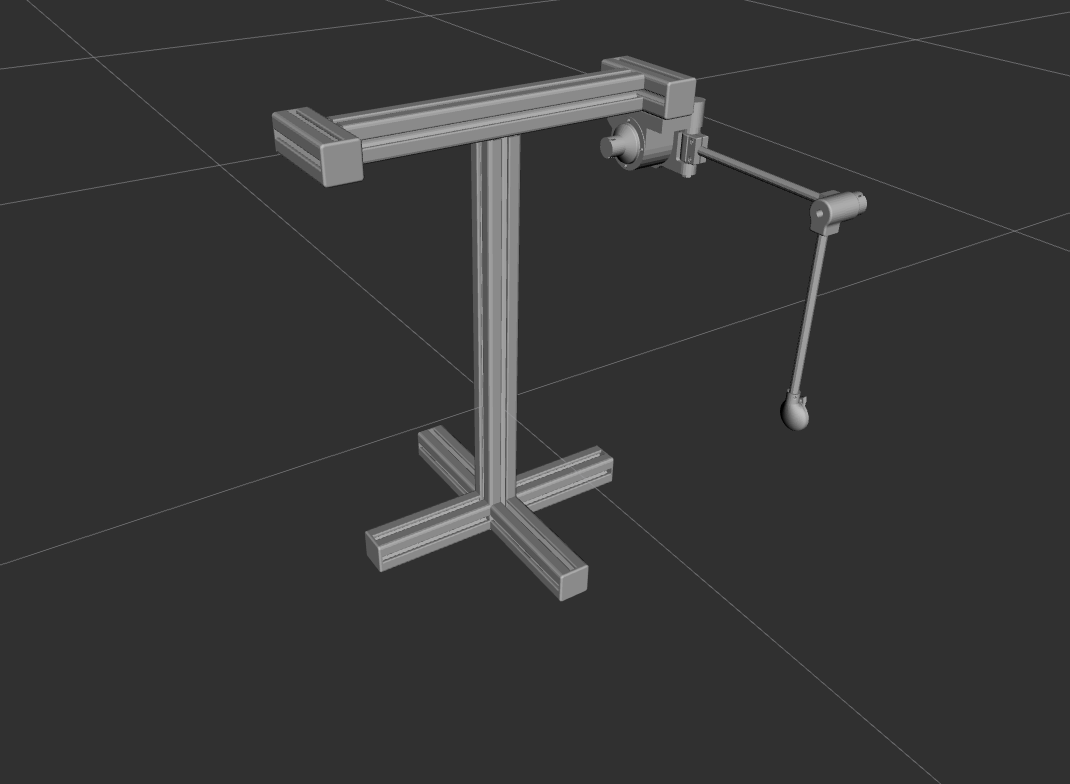
\includegraphics[width=0.75\linewidth]{figures/mtm_sdf_model.png}
    \caption{SDF model of MTM}
    \label{fig:mtm_sdf_model}
\end{figure}

\subsection{MTM Data Streaming and filtering}

The MTM node's primary purpose is to process incoming sensor data and broadcast it into the \texttt{ROS2} workspace in a usable format. The following topics are published into the \texttt{ROS2} workspace from the MTM:

---

The MTM node's primary purpose is to process incoming sensor data and broadcast it into the \texttt{ROS2} workspace in a usable format. The following topics are published into the \texttt{ROS2} workspace from the MTM:

---

\begin{table}[h!]
    \centering
    \caption{MTM \texttt{ROS2} Topics}
    \label{tab:mtm_ros2_topics}
    \begin{tabular}{|l|l|p{5cm}|} % Changed to p{5cm}
        \hline
        \textbf{Topic Name} & \textbf{Topic Type} & \textbf{Description} \\
        \hline
        \texttt{mtm\_joint\_states} & \texttt{sensor\_msgs/msg/JointState} & Current angular positions for all robotic arm joints. \\
        \hline
        \texttt{mtm\_raw\_values} & \texttt{std\_msgs/msg/Float32MultiArray} & Unfiltered raw sensor data for debugging. \\
        \hline
        \texttt{12target\_pose} & \texttt{sensor\_msgs/msg/JointState} & Calculated Cartesian (x, y, z) position of the end-effector in meters. \\
        \hline
    \end{tabular}
\end{table}

\subsection{MTM to PSM Communication Protocol}

As previously established in Section 4.1, there are two separate paths for data communication between the MTM and the PSM: the direct communication path and the path utilizing the SDF model as an intermediary.

A critical aspect of both communication paths is ensuring \textbf{Quality of Service (QoS)} protocol matching. QoS allows for the definition of how topics are communicated between nodes. Ensuring that communicating nodes utilize appropriate and compatible QoS protocols is essential for software reliability and robustness. For this research, the QoS reliability and queue depth were modified to ensure proper message delivery.

Initially, an issue arose with the communication protocol between the SDF model and the PSM node. Data streamed from the SDF model was published to the \texttt{/model\_pose} topic. When this data was plotted, it exhibited high quality with zero latency or lag. However, when the PSM topic \texttt{/psm\_joint\_telemetry} subscribed to \texttt{/model\_pose}, a significant loss of data occurred, resulting in lag and stuttering. This led to unacceptable system performance. After extensive diagnostics, the data performance was improved by drastically increasing the publishing rate from 100\,Hz to 1000\,Hz, increasing the queue depth from 10 to 20, and applying the following QoS profile:

\begin{itemize}
    \item \textbf{Reliability:} \texttt{RELIABLE}
    \item \textbf{History (Depth):} 20
    \item \textbf{Durability:} \texttt{VOLATILE}
    \item \textbf{Lifespan:} Infinite
    \item \textbf{Deadline:} Infinite
    \item \textbf{Liveliness:} \texttt{AUTOMATIC}
    \item \textbf{Liveliness lease duration:} Infinite
\end{itemize}

Increasing the publishing rate to such a drastic level required careful memory consideration to avoid overwhelming the limited memory of the PSM's Teensy 4.1. As a result, the \texttt{model\_pose} message type was changed from a \texttt{JointTelemetry} message type to a \texttt{JointState} message type to reduce memory strain.

\begin{figure}
    \centering
    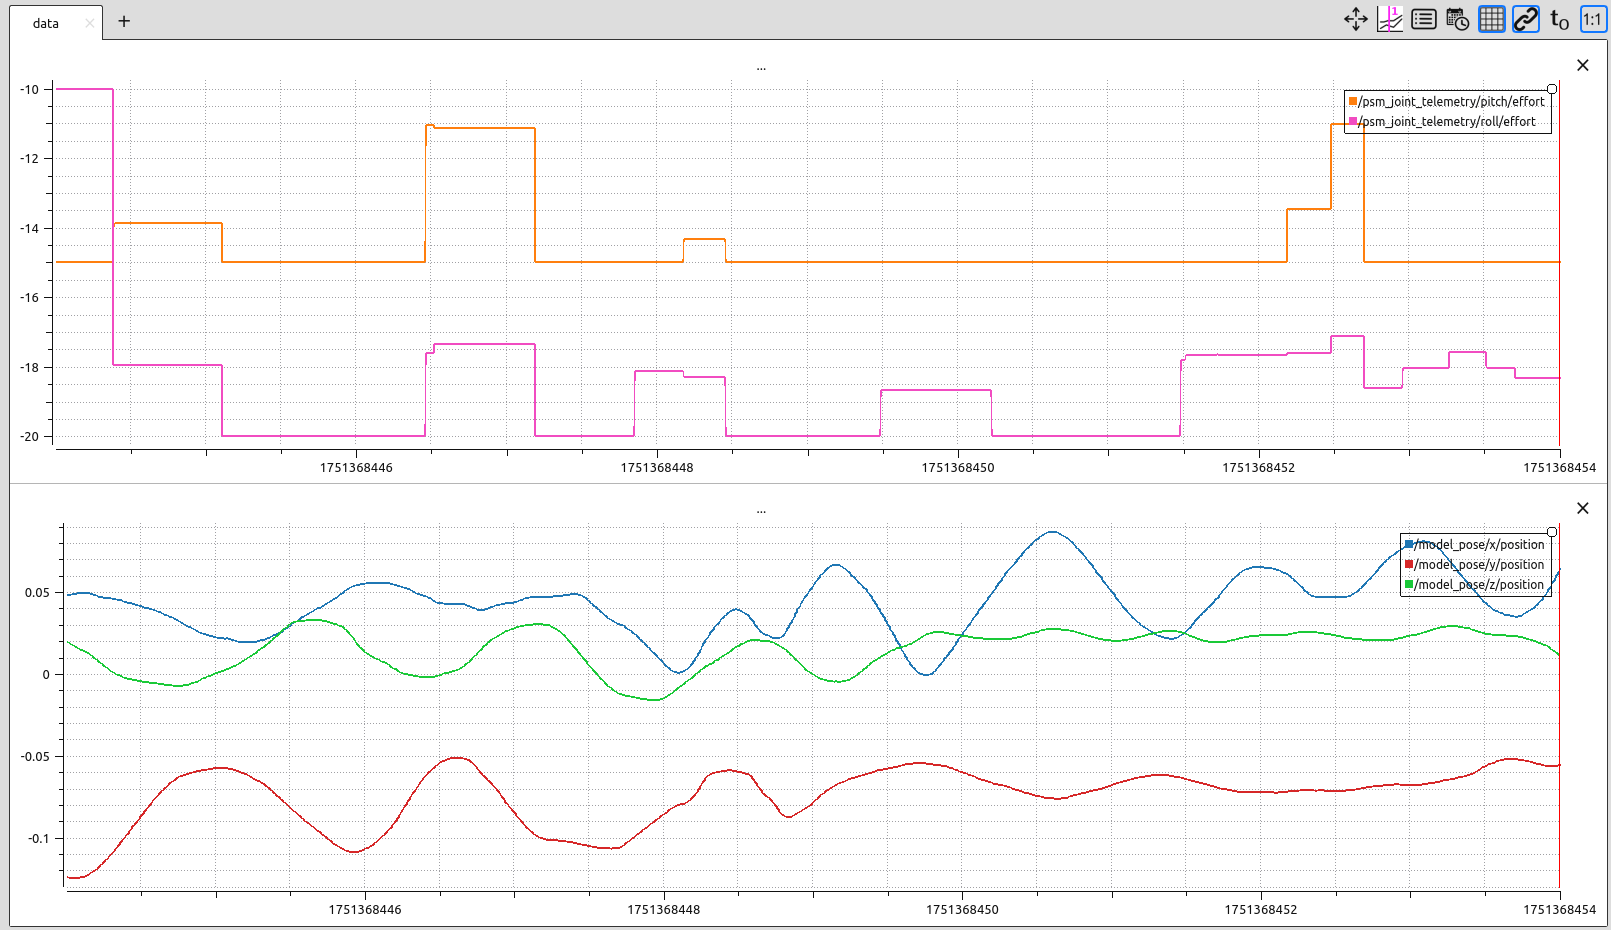
\includegraphics[width=0.5\linewidth]{figures/bad_data.png}
    \caption{Enter Caption}
    \label{fig:bad_data_placeholder}
\end{figure}

\subsection{PSM Software}

The PSM software node's primary responsibility is the control of the physical PSM system. While this task may appear simple on the surface, its implementation was quite complex, requiring several different software components to work together cohesively.

The PSM node had two primary modes:

\begin{itemize}
    \item \textbf{Target Mode:} In this mode, the PSM node received target joint angles from the MTM node and the Joint Publisher Node. The PSM would then drive the system to these target angles using a control algorithm. This mode was primarily used for the normal operation of the PSM.
    \item \textbf{Verification Mode:} In this mode, the PSM followed a predetermined trajectory to verify the system's performance. This mode was primarily used for testing and validation purposes.
\end{itemize}

In both modes, the primary codebase remained the same, consisting of a \texttt{main.cpp} file and multiple helper files. The primary difference between the modes was the subscription to the target pose topic. In Target Mode, the PSM node subscribed to the \texttt{/mtm\_target\_pose} topic, while in Verification Mode, it generated its own target pose trajectory and was completely self-contained.

In Target Mode, the PSM node subscribed to two different topics. For overall positioning of the system, it subscribed to the \texttt{/target\_pose} topic generated by the Joint Publisher Node. This topic provided the target position in an \texttt{x, y, z} format. The PSM node then used this target position to calculate the necessary joint angles to achieve this position. Additionally, to determine the desired tool angles, it subscribed to the \texttt{/mtm\_joint\_states} topic. This topic provided the current gimbal angles of the MTM system, which were used to calculate the necessary joint angles for the PSM system.

In an effort to modularize the codebase and improve readability the PSM software was broken up into several different files, each responsible for a specific functionality. The following is a list of the primary files in the PSM software codebase:

\begin{itemize}
    \item \textbf{config.h}: The file acts as a central repository for all configuration parameters used throughout the PSM software. It contains definitions for various constants, such as the number of axes, pin definitions, motor IDs, and other parameters that can be easily modified to adjust the system's behavior.
    \item \textbf{LQR.cpp}: This file implements the Linear-Quadratic Regulator (LQR) and Linear-Quadratic-Integral (LQI) control algorithms. These controllers are used to calculate the necessary control inputs for the roll and pitch axes of the robotic arm, ensuring stable and precise movements.
    \item \textbf{PID.cpp}: This file contains the implementation of a standard PID (Proportional-Integral-Derivative) controller. It provides an alternative control strategy that can be used for the various axes of the robot, calculating control values based on the error between the target and actual positions.
    \item \textbf{axis\_conversion.cpp}: This file provides functions to convert between encoder counts and physical units such as angles (degrees) and linear positions (mm). This is essential for interpreting sensor data and commanding the motors accurately.
    \item \textbf{encoder\_lp.cpp}: This file implements a low-pass filter for the encoder readings. This is used to smooth out noisy encoder signals, providing a cleaner and more stable measurement of the robot's position.
    \item \textbf{encoder\_reader.cpp}: This file is responsible for reading the raw data from the motor encoders. It defines the encoder objects and provides a function to read the encoder counts for each axis.
    \item \textbf{gain\_schedule.cpp}: This file implements a gain scheduling algorithm for the LQR-based controllers. It contains precomputed gain tables and uses interpolation to select the appropriate controller gains based on the current roll and pitch angles of the robot.
    \item \textbf{helper\_functions.cpp}: This file contains various utility functions used throughout the project. These include functions for publishing debug messages, mapping gimbal angles to servo angles, and handling critical errors.
    \item \textbf{homing.cpp}: This file implements the homing sequence for the motors. This routine is responsible for moving the robot to a known starting position, which is crucial for accurate and repeatable operation.
    \item \textbf{main.cpp}: This is the main entry point of the application. It initializes the ROS 2 node, sets up subscribers and publishers, and contains the main control loop that reads sensor data, calculates control inputs, and commands the motors.
    \item \textbf{psm\_joint\_angles.cpp}: This file contains the inverse kinematics calculations for the patient-side manipulator (PSM). It computes the required joint angles for the roll, pitch, and insertion axes based on a target position in Cartesian space.
    \item \textbf{ramp.cpp}: This file provides a function to generate a smooth motion profile, or ramp, between a current and target angle. This is used to prevent jerky movements and ensure the robot moves in a controlled manner.
\end{itemize}

\section{System Identification}

For this research, proper controller design was paramount. However, a high-performance controller could not be designed without a fundamental understanding of the system's dynamics. To achieve this, a robust system identification scheme was developed.

The two primary joints of interest were the roll and pitch joints. These joints exhibited complex system dynamics and a high degree of nonlinearity. An exact system identification approach was tailored to each joint's unique dynamics.

\subsection{Roll Joint Open loop Step Response}

The roll joint can be mechanically described as a pendulum. Perturbations applied to the system move the joint away from its $0^\circ$ position, but when the perturbation ceases, gravitational forces return the joint to its $0^\circ$ position. The system was also determined to have a fairly consistent and predictable transfer function. Specifically, when the brushless motor was driven at a specific voltage, the resulting positional change of the system was consistent across trials. As a result of these factors, a step response characterization was deemed an excellent method for system identification.

A step response characterization is a common system identification method in control engineering. In this technique, the system's input is abruptly changed from one value to another, and the resulting system response is measured and used to characterize the system's dynamics.

For the roll axis, a very lightly tuned PID controller was initially employed to drive the system to the intended point of characterization. A predetermined delay allowed the system to settle into a stable state. Upon completion of this delay, the current motor voltage value was stored, then scaled by a factor of 1.1 before being sent to the motor. Both the motor voltage input over time and the positional output of the roll joint over time were recorded. This system response data was saved as a CSV file and subsequently loaded using a custom MATLAB script. This script parsed the data and then fitted a second-order transfer function to the system response using MATLAB's \texttt{tfest} command. Finally, state-space matrices could then be extracted from this transfer function using MATLAB's \texttt{ss} command.



\subsection{Closed loop excitation through PRBS}

Initial characterization of the pitch subsystem used a similar approach to the roll subsystem. A step response was applied, and the resulting response was used to characterize the system. However, several issues were found with the step response characterization of the pitch subsystem.

Due to the mechanical nature of the joint, the pitch subsystem's response was highly nonlinear. A slight change in voltage applied to the motor resulted in large changes in the pitch system's position, and this behavior was not consistent between trials. The same change in motor voltage would not result in the same system response. Additionally, when a small increase in voltage was applied to a stable system position, the pitch subsystem would drive to the end of its range of motion and contact the hard stop. This overshooting was a result of the pitch subsystem's extremely sensitive system response as its angle increased. This sensitivity was a direct consequence of the mechanical design of the pitch subsystem, where the force applied by the gravity compensation system drastically reduced as the angle of the pitch subsystem increased.

As a result of these complexities, a different approach had to be implemented. Due to the difficulties in maintaining the pitch subsystem within its intended range of motion, it was deduced that system identification needed to be conducted under closed-loop system control.

For this system identification technique, a light PD controller was applied to the system. The system was then commanded to its intended characterization point. Upon a predetermined settling time, the control input was then excited with a Pseudo-Random Binary Sequence (PRBS).

PRBS is a control signal excitation technique in which the control input is randomly fluctuated by a set amplitude at pseudo-random, predetermined intervals. By exciting the control input, the resulting behavior and system dynamics could be observed while the aforementioned PD controller attempted to bring the system back to its setpoint. Key considerations in closed-loop PRBS excitation are ensuring that the amplitude of the excitation is sufficient to bring the system off its setpoint and overcome noise, while also ensuring that the amplitude of the excitation does not overpower the controller and drive the system off its setpoint. Additionally, the intervals between the fluctuations of the excitation need to be chosen such that the system's dynamics are excited across a variety of frequencies.

To ensure that the system undergoes excitation at all critical frequencies multiple times, the PRBS characterization was run for an extended period. Trials typically lasted 30-660 seconds. During these trials, the pitch subsystem's input voltage and resulting position were continuously recorded. This output data was saved as a CSV file, and an additional MATLAB script was used to perform a mathematical characterization of the system.

Similarly to the roll subsystem, the recorded output of the pitch subsystem was loaded into a MATLAB script, and a variety of system identification techniques were applied to the data.

From these results, it was determined that a 4th-order transfer function estimation was the best method for characterizing the system.

After a 4th-order transfer function was fitted to the system using the MATLAB \texttt{tfest} command, the state-space matrices were extracted using the \texttt{ss} command. The estimated model's accuracy was then determined by comparing the actual system behavior based on the input to the predicted system behavior based on the system input using the MATLAB \texttt{compare} command.

From this comparison, it was determined that the model accuracy was quite low when compared to the real system response based on the input. However, when a controller was designed around this model estimation, the actual system performance was quite good. So, while this poor system estimation may point towards some underlying issues in the system identification technique, it ultimately resulted in a high-performing controller, which was the ultimate goal of this research.


\subsection{Multi-point System Identification}

Due to the kinematics of the system, the force required of the motors at various joint positions will vary. As the roll angle diverges farther from 0 in both the negative and positive direction, there is an increase in gravitational forces seen by the actuators, and as a result, the voltage applied to the motor would need to be increased accordingly. This trend is theoretically illustrated in Figure~\ref{fig:roll_voltage_trend}.

\begin{figure}[htbp]
    \centering
    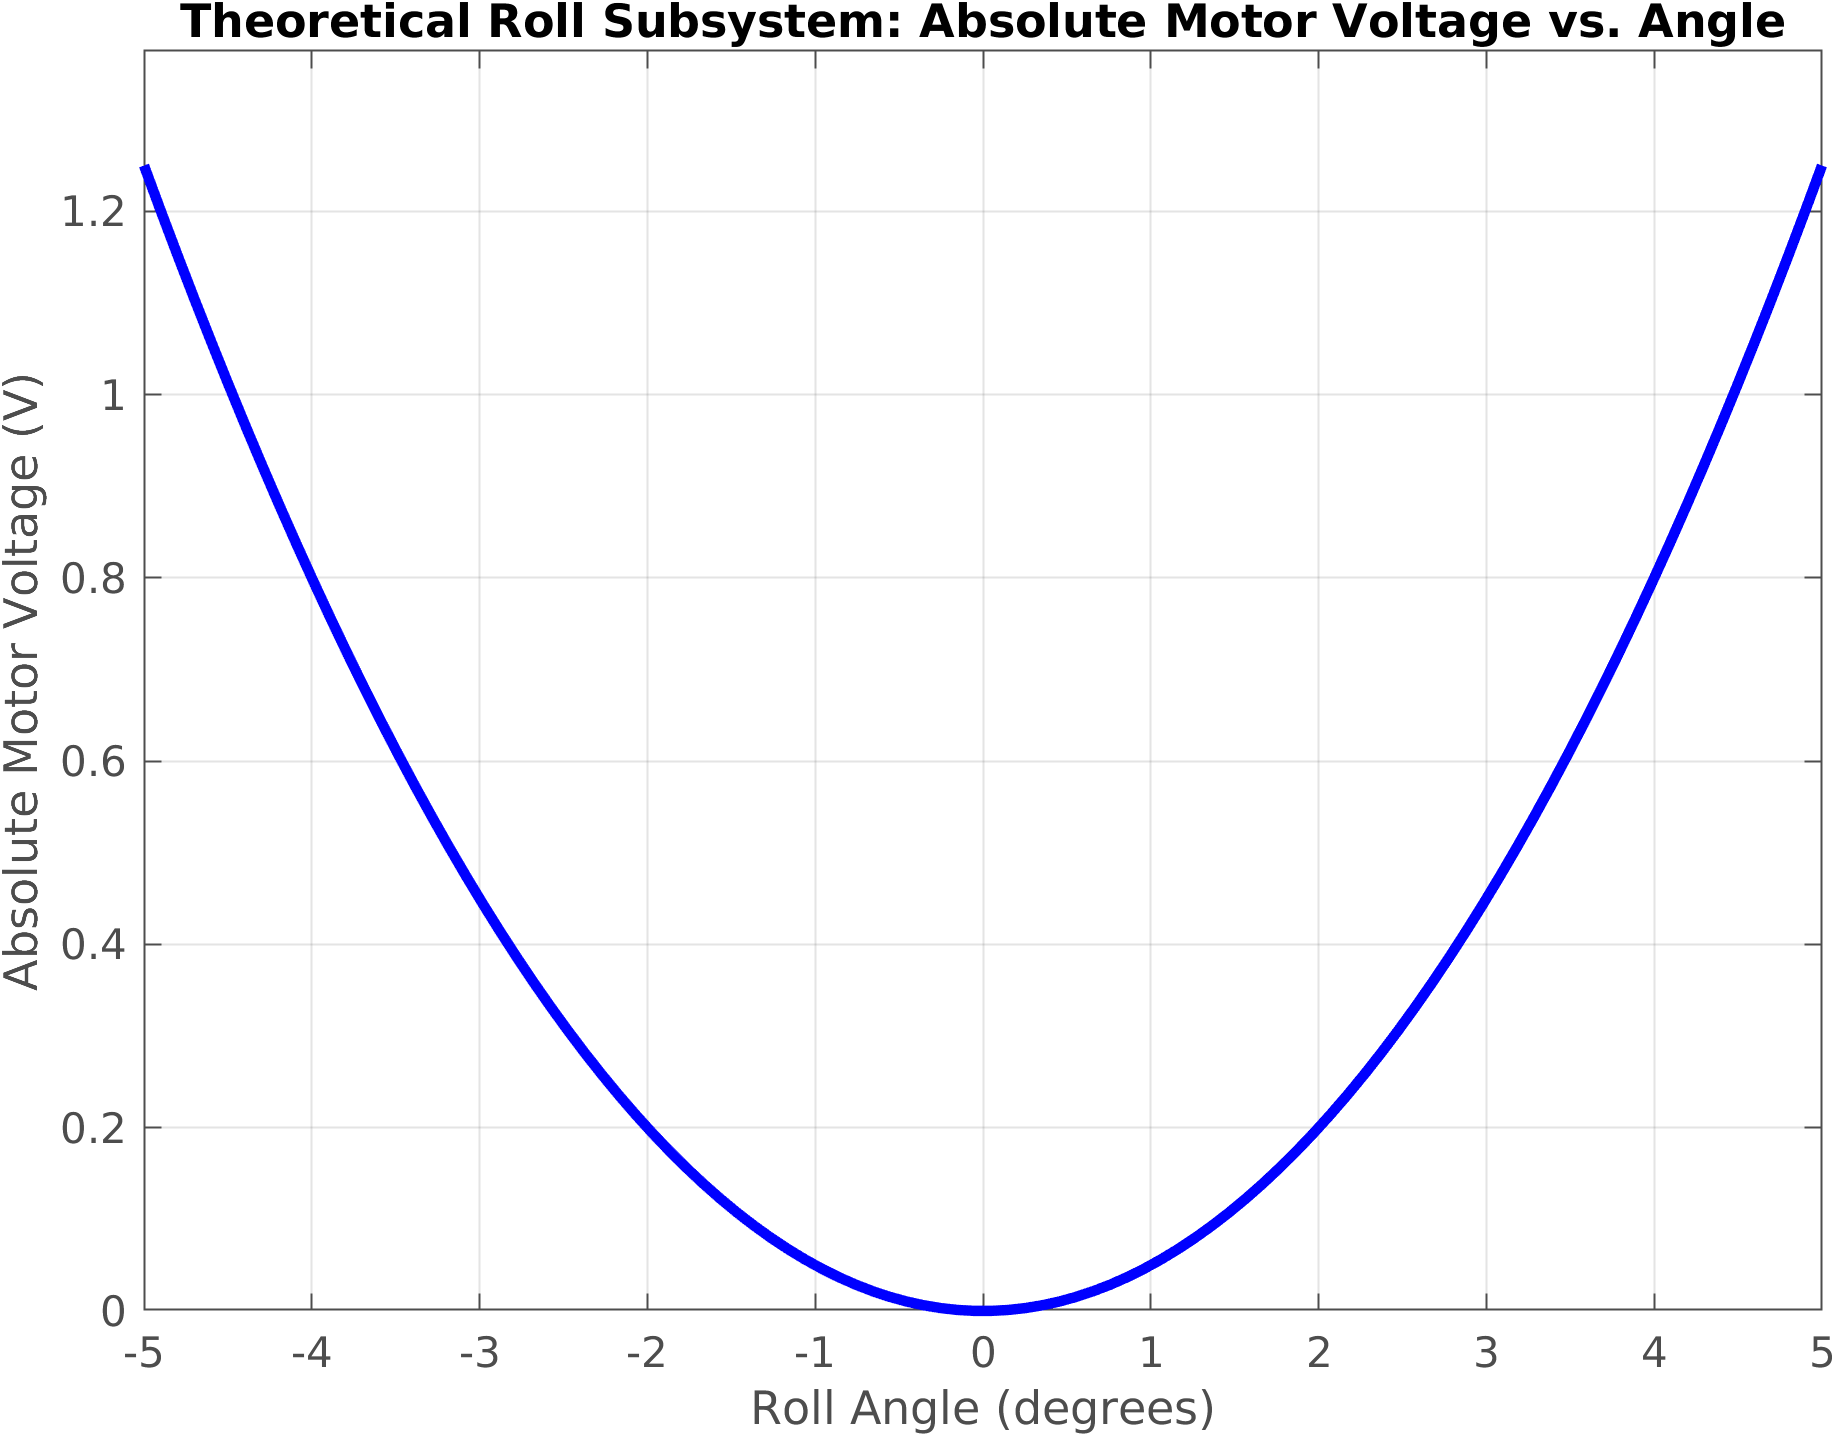
\includegraphics[width=0.8\textwidth]{figures/Roll_Subsystem_Theoretical_Trend.png}
    \caption{Theoretical trend of absolute motor voltage required for the roll subsystem as a function of roll angle.}
    \label{fig:roll_voltage_trend}
\end{figure}

For the pitch subsystem, the force required by the actuator actually decreases as the joint moves through its range of motion from -30 degrees to 30 degrees. The theoretical voltage required for the pitch subsystem across its range of motion is shown in Figure~\ref{fig:pitch_voltage_trend}.

\begin{figure}[htbp]
    \centering
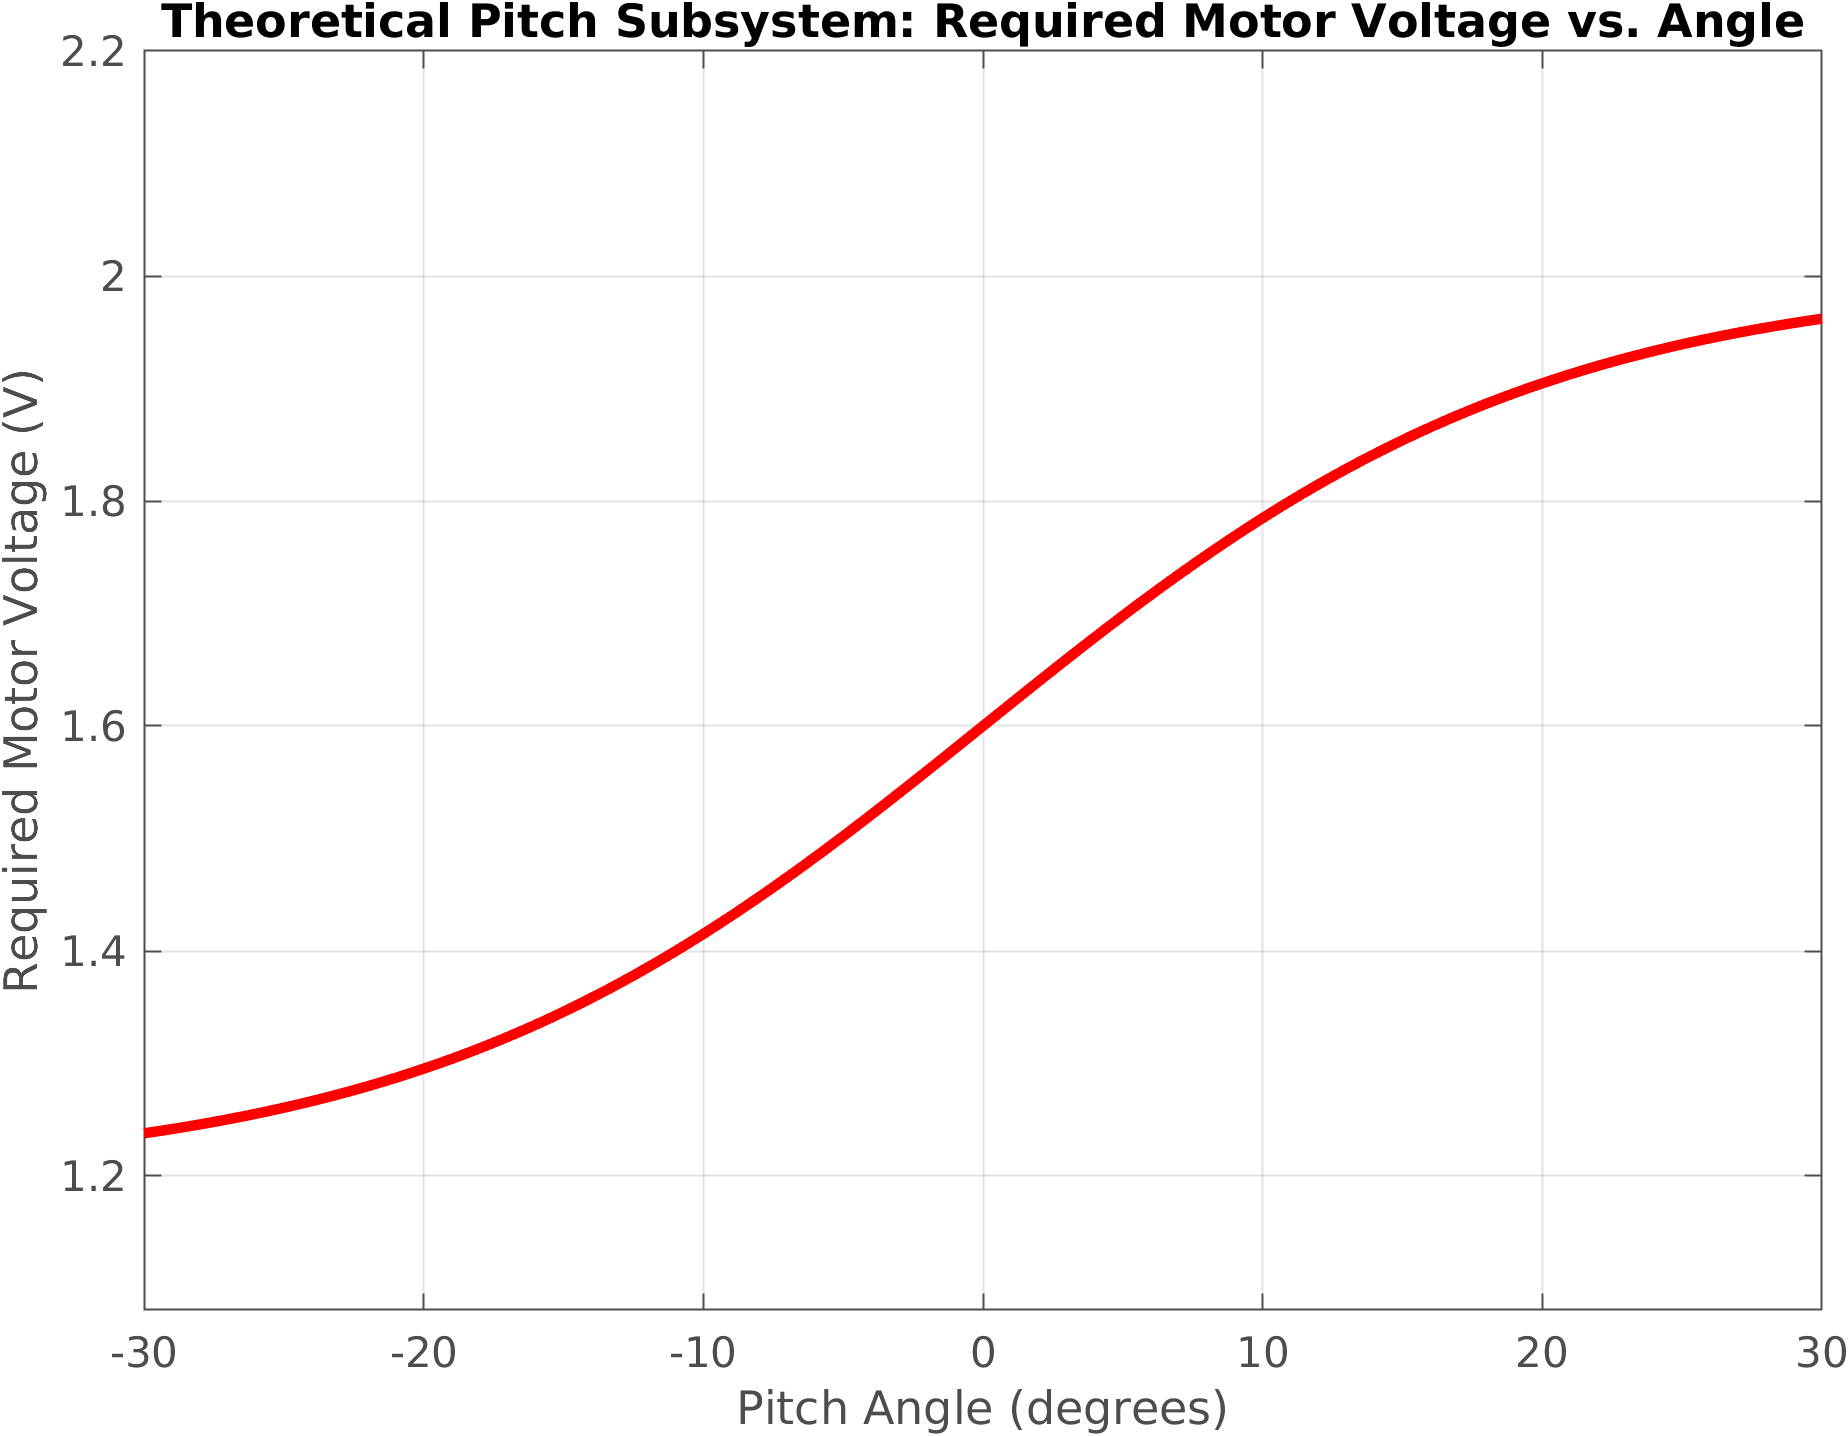
\includegraphics[width=0.8\textwidth]{figures/Pitch_Subsystem_Theoretical_Trend.png}
    \caption{Theoretical trend of required motor voltage for the pitch subsystem as a function of pitch angle.}
    \label{fig:pitch_voltage_trend}
\end{figure}

Additionally, complexities are added to the system dynamics when one realizes that the force required by the roll subsystem is also coupled to the pitch subsystem's position. As the pitch subsystem's angle is increased, the force required by the roll subsequently changes due to the system's center of mass changing position.

Similarly, the force required by the pitch subsystem varies with the position of the roll subsystem. As the roll subsystem diverges from the 0 point, the force required by the pitch subsystem lessens as it stays farther from its default position (normal to the gravitational force vector).

The combination of these factors necessitated the need for a more complex controller strategy in which the controller gains varied in accordance with the system position. The idea of this improved controller was that each joint's gains would vary with the current position of each subsystem.

This adaptive controller algorithm would require the characterization of the system at multiple points of the system's position. It was decided that 9 characterization points would be used for each joint of the subsystem. The pitch would be varied from $-15^\circ$, $0^\circ$, $15^\circ$ and the roll subsystem would vary from $-20^\circ$, $0^\circ$, $20^\circ$. This resulted in the following grid of 9 characterization points:

\begin{table}[htbp]
    \centering
    \caption{Grid of 9 Characterization Points for System Identification}
    \label{tab:characterization_points}
    \begin{tabular}{c|ccc} % c for the first column, then 3 c's for the data columns
        \multicolumn{1}{c}{} & \multicolumn{3}{c}{\textbf{Roll Angle ($^\circ$)}} \\
        \cmidrule(lr){2-4} % Line under Roll Angle
        \textbf{Pitch Angle ($^\circ$)} & \textbf{-20} & \textbf{0} & \textbf{20} \\
        \midrule % Line separating headers from data
        \textbf{-15} & $(-15, -20)$ & $(-15, 0)$ & $(-15, 20)$ \\
        \textbf{0}   & $(0, -20)$   & $(0, 0)$   & $(0, 20)$   \\
        \textbf{15}  & $(15, -20)$  & $(15, 0)$  & $(15, 20)$  \\
        \bottomrule
    \end{tabular}
\end{table}

Once the necessary characterization points were established, the system needed to be identified at each of these points for each joint, resulting in the necessary system identification procedures. The actual system identification process was fairly straightforward. The previously established strategy for each joint was used; the only difference was that the positional setpoint for each characterization point varied to ensure the joint not being characterized remained at the necessary setpoint. The controller designed around the $(0,0)$ characterization point was used. While it was found that the dynamic performance of the controller designed around the $(0,0)$ setpoint degraded as the system diverged farther from the original linearization point, this controller performed well enough in the case of a static setpoint that it could be used to hold the extreme angles required by the multi-point system identification.

Once the necessary characterization points were established, the system needed to be identified at each of these points for each joint, resulting in the necessary system identification procedures. The actual system identification process was fairly straightforward. The previously established strategy for each joint was used; the only difference was that the positional setpoint for each characterization point varied to ensure the joint not being characterized remained at the necessary setpoint. The controller designed around the $(0,0)$ characterization point was used. While it was found that the dynamic performance of the controller designed around the $(0,0)$ setpoint degraded as the system diverged farther from the original linearization point, this controller performed well enough in the case of a static setpoint that it could be used to hold the extreme angles required by the multi-point system identification.

Upon the completion of each system identification trial, the resulting system response was saved in a CSV file under the following format: \texttt{IDENTIFIEDJOINT\_ROLLANGLE\_PITCHANGLE.csv}. A MATLAB script was then used to parse each of these files, identify the system at that point, and store and plot the system identification results.

\section{Controller Theory and Design}
The controller design was paramount to this research; a high emphasis was placed on system performance, and proper controller design would directly drive this. As a result, a large amount of effort was put into both the design and tuning of the controller.

\subsection{Original PID Controller}

The system originally utilized a very basic PID controller. Tuning was conducted with the Ziegler-Nichols method, and the following gains were found for each subsystem:

\begin{table}[htbp]
    \centering
    \caption{Ziegler-Nichols PID Gains for Roll and Pitch Subsystems}
    \label{tab:pid_gains}
    \begin{tabular}{l c c c}
        \toprule
        \textbf{Subsystem} & \textbf{$k_p$} & \textbf{$k_i$} & \textbf{$k_d$} \\
        \midrule
        Roll               & 35             & 50             & 5              \\
        Pitch              & 60             & 110            & 5              \\
        \bottomrule
    \end{tabular}
\end{table}

However, with these values, when full PID control was used, the system would rapidly vibrate, leading to uncontrolled system behavior and unacceptable noise and vibration. Because of this, the original system was only ever used with PD control, and its performance suffered greatly. Following sinusoidal trajectories, it would frequently undershoot or overshoot the setpoint and responded poorly to perturbations. As a result, an improved controller method needed to be developed.


\subsection{Model Predictive Control (MPC)}

Initially, several types of controllers were considered for this system. Model Predictive Control (MPC) was initially considered, as the system was already partially modeled in the form of an SDF model. MPC uses a dynamic model of the system to predict system behavior and determine a cost-optimal control input based on the model dynamics. While this control technique would result in extremely robust and optimal control, two factors prevented its utilization. First, the system model was a purely geometrical model, only accounting for the mass and inertia properties. Internal dynamics, such as frictional forces, were not considered, and the complexities of modeling such behavior were daunting. Secondly, MPC requires high computational power to simultaneously run and predict the model's behavior. This system utilized low-cost hardware with limited computational resources and, as a result, lacked the computational power to perform MPC.

\subsection{Gain Scheduling and Adaptive Control}

It was clear that due to varying system dynamics across the system's range of motion, adaptive control or gain scheduling would be a very valuable asset in improving system performance. Adaptive control involves online estimation of unknown or time-varying system parameters, or direct adjustment of controller parameters based on real-time performance feedback. In contrast, gain scheduling is a pre-programmed approach where controller parameters are adjusted based on a known, measurable "scheduling variable."

With relatively little additional computational power and complexity, the control gains could be calculated and interpolated based on the system's position, making gain scheduling an excellent candidate for improving system performance.



\subsection{LQR and LQI Control}

Linear Quadratic Regulator (LQR) control and Linear Quadratic Integral (LQI) control are cost-optimal control algorithms that minimize a quadratic cost function. LQI control extends the efforts of LQR control by incorporating integral action, which reduces steady-state error and improves system performance.

Both of these control methods are well-suited to this research as they achieve a good balance of high system performance with minimal control efforts. LQR control was chosen for the roll joint, as it was found that its performance was more than adequate for the system. However, during testing of the pitch subsystem, it was found that the system was consistently undershooting the desired positional setpoint. It was found that an LQI controller would minimize this steady-state error and drastically improve performance.

The objective of LQR control is to find a control input $\mathbf{u}(t)$ that minimizes the following quadratic cost function:
$$ J_{LQR} = \int_{0}^{\infty} (\mathbf{x}^T(t) Q \mathbf{x}(t) + \mathbf{u}^T(t) R \mathbf{u}(t)) \, dt $$
where:
\begin{itemize}
    \item $\mathbf{x}(t)$ is the state vector.
    \item $\mathbf{u}(t)$ is the control input vector.
    \item $Q$ is a positive semi-definite weighting matrix for the states, penalizing deviations from the desired state (often the origin).
    \item $R$ is a positive definite weighting matrix for the control inputs, penalizing control effort.
\end{itemize}

For LQI control, the system is augmented with an integral of the error, and the cost function is similarly minimized. If $\mathbf{e}_I(t)$ represents the integral of the output error, the augmented state $\mathbf{x}_{aug}(t)$ includes the original states and the integral error. The cost function for LQI is then:
$$ J_{LQI} = \int_{0}^{\infty} (\mathbf{x}_{aug}^T(t) \tilde{Q} \mathbf{x}_{aug}(t) + \mathbf{u}^T(t) R \mathbf{u}(t)) \, dt $$
where $\tilde{Q}$ is the augmented weighting matrix for the states, including a penalty on the integral error to drive it to zero.


\subsection{Feedforward Control}

Feedforward control is a control method which attempts to anticipate changes or disturbances to the system's input. It was theorized that a feedforward control strategy could further reduce any remaining steady-state error in the pitch subsystem.

In order for feedforward control to be implemented, a model of the system must be constructed in the form of a specific matrix known as the $B^\dagger$ matrix. The $B^\dagger$ matrix is formulated through the Moore-Penrose pseudoinverse. It is formulated as follows:

Let $B$ be an $m \times n$ real or complex matrix. Its Singular Value Decomposition (SVD) is given by:
$$B = U \Sigma V^T$$
where:
\begin{itemize}
    \item $U$ is an $m \times m$ unitary (or orthogonal for real matrices) matrix whose columns are the left singular vectors of $B$.
    \item $\Sigma$ is an $m \times n$ rectangular diagonal matrix with non-negative real numbers on the diagonal, called the singular values of $B$, typically arranged in decreasing order.
    \item $V^T$ is an $n \times n$ unitary (or orthogonal for real matrices) matrix whose rows are the right singular vectors of $B$. ($V$ is the matrix of right singular vectors).
\end{itemize}

The \textbf{Moore-Penrose pseudoinverse} of $B$, denoted $B^\dagger$, is then defined as:
$$B^\dagger = V \Sigma^\dagger U^T$$
where $\Sigma^\dagger$ is an $n \times m$ matrix formed by taking the reciprocal of each non-zero singular value on the diagonal of $\Sigma$, and then transposing the matrix.

The pseudoinverse $B^\dagger$ is unique and provides a "least squares" solution to linear equations. For a system $Bx = y$, if an exact solution doesn't exist, $x = B^\dagger y$ provides the solution that minimizes $||Bx - y||_2$.

For the purpose of this research, this matrix could be calculated via the MATLAB command \texttt{pinv}. This command, when applied to the identified $B$ matrix from the system identification procedure, would result in the $B^\dagger$ matrix.


This procedure was conducted for each of the characterization points previously discussed. Upon calculation of the $B^\dagger$ matrix, this matrix is used to calculate $u_{ff}$ by multiplying the $B^\dagger$ matrix (pseudoinverse of the input matrix) with the sum of the system's $A$ matrix multiplied by the reference state and the time derivative of the reference state. This $u_{ff}$ is then scaled by a factor $\lambda$, which can be tuned from $0$ to $1.0$ to adjust the feedforward element of the controller.

The ultimate result of this control effort is to proactively cancel anticipated system dynamics and generate better system performance.

\subsection{Comprehensive Control Strategy}


The final controller for the system was a resulting combination of several of the control strategies previously discussed. Ultimately, for the roll joint, it was found that gain scheduling with an LQR controller provided adequate system performance. However, for the pitch subsystem, this method needed to be improved upon due to consistent steady-state error in the form of target undershooting. To remedy this, an LQI controller with feedforward implementation and gain scheduling was employed. These strategies led to drastic improvements in system performance.